\documentclass[conference]{IEEEtran}
\usepackage{graphicx}
\usepackage{booktabs}
\usepackage{amsmath}
\usepackage{url}
\usepackage{cite}
\graphicspath{{../figures/}{figures/}}

\begin{document}

\title{Load-Blind Latency Models Pick the Wrong Edge Node:\\
A Measurement Study of Game Server Placement}

% TODO: full registered names of all five authors, same order as agreed.
\author{\IEEEauthorblockN{Ankam Charan Teja, Aranya Roy, Akshit Singh, Nikhil, Yash}}

\maketitle

\begin{abstract}
Edge placement algorithms choose a node with an analytical latency model,
propagation delay plus data size over bandwidth, that has no term for server
load. Edge nodes are small, so a crowded edge can add more delay inside the
server than its proximity saves, and because placement work is usually
evaluated in simulators built on the same model, the error does not show. We
measure it. On an emulated four-node edge--cloud testbed (0.5, 1, 2 and 4
cores at 5, 15, 30 and 40\,ms round-trip time) running a real multiplayer
game server and up to 160 protocol-level bot players, we record network,
transport, server-process and in-game latency concurrently. The ICMP round
trip never moves more than 0.3\,ms from its configured value, while the 95th-percentile in-game
latency of the smallest node rises from 15\,ms at 40 players to 6.7--8.6\,s at
60. We fit a closed-form M/M/1 model and a gradient-boosted tree model to
two replicates of the load grid, compute each model's optimal placement for
40 to 160 players, and deploy every placement for real. The load-blind
placement leaves its worst players at 18--30\,s from 80 players on; both
load-aware placements stay at 20--39\,ms. The learned model predicts latency
best (median error 0.9\,ms against 1.8\,ms and 5.8\,ms, and 1.2\,ms on a
held-out third replicate) but, on these scenarios, does not place better than
the fitted closed form. Run as a live controller on the same schedule of
players, the load-blind model never moves a match and its worst players sit
at a median of 1.06\,s; the learned model keeps them at a median of 33\,ms. When one node
silently loses half its CPU, only a variant that corrects itself from live
measurements moves players off it.
\end{abstract}

\section{Introduction}

Putting a game server at the network edge shortens the path to its players.
Edge nodes, however, are small: a base-station or street-cabinet server has a
fraction of a data-centre machine's compute and cannot scale out. When enough
players are placed on one, its CPU saturates and the delay added inside the
server grows without bound, while the network delay it saves is fixed.

Placement algorithms rank candidate nodes with an analytical model of latency,
\begin{equation}
  \textit{latency} = \textit{propagation delay} + \frac{\textit{data size}}{\textit{bandwidth}},
  \label{eq:analytical}
\end{equation}
which has a term for distance and a term for bandwidth and none for load. The
error this causes is hard to see in the literature because placement policies
are mostly evaluated numerically or in discrete-event simulators such as
iFogSim~\cite{gupta2017ifogsim}, YAFS~\cite{lera2019yafs},
EdgeCloudSim~\cite{sonmez2018edgecloudsim} and
PureEdgeSim~\cite{mechalikh2021pureedgesim}. A recent taxonomy of microservice
placement in fog computing states the gap directly: the majority of works
evaluate by numerical analysis or simulation and fail to validate on real
testbeds, so resource contention among services is not accurately
captured~\cite{pallewatta2023taxonomy}.

This paper measures that error instead of modelling it. Our contributions:
\begin{itemize}
  \item an emulated edge--cloud testbed running a real game server binary and
        protocol-level clients, with latency measured at four depths at once,
        so delay is attributed to a layer rather than inferred;
  \item a labelled dataset mapping (node, load) to measured tail latency,
        three replicates (one held out for testing), released with the code;
  \item an end-to-end comparison in which each latency model's optimal
        placement is deployed and measured, so models are graded by a clock
        rather than by each other;
  \item a live placement controller on the same testbed, run under the
        load-blind and the learned model on the same schedule of players, including a node that loses
        half its CPU mid-run without any model being told.
\end{itemize}

\section{Related Work}

\textbf{Service placement in fog and edge.} Surveys of the service placement
problem~\cite{aitsalaht2019overview} and of microservice
placement~\cite{pallewatta2023taxonomy} catalogue objectives, constraints and
algorithms. Latency is commonly modelled as in (\ref{eq:analytical}), with
server-side processing either omitted or taken as a constant per request.

\textbf{Simulators.} iFogSim~\cite{gupta2017ifogsim} and
EdgeCloudSim~\cite{sonmez2018edgecloudsim} build on CloudSim;
YAFS~\cite{lera2019yafs} on a discrete-event library and network graphs;
PureEdgeSim~\cite{mechalikh2021pureedgesim} targets large heterogeneous
deployments. All compute latency from configured link and processing
parameters. They are indispensable for scale, but an algorithm evaluated in
them is graded by the same assumptions it was designed with.

\textbf{Closing the simulator gap.} SimTune~\cite{tuli2022simtune} uses a
low-fidelity surrogate model to tune a high-fidelity simulator's parameters
against a real edge--cloud platform, improving energy and response time of
resource management. We take the opposite route: we keep no simulator, learn
the load--latency relationship directly from measurements of an interactive
workload, and evaluate on worst-player tail latency rather than mean
response time.

\textbf{Queueing-aware placement.} Closed-form queueing terms such as
$s/(1-u)$ for utilization $u$ are the standard way to add load to a latency
model. We include a fitted M/M/1 model as the strongest closed-form baseline
rather than compare only against (\ref{eq:analytical}).

\section{Testbed and Method}

\subsection{Topology}
Five containers on one host are wired by containerlab: a client node and four
candidate servers. Distance is emulated with Linux \texttt{netem}, half the
target delay on each end of each link; compute is capped with a cgroup CPU
quota on disjoint CPU sets. Table~\ref{tab:nodes} lists the nodes; the RTT is
measured with \texttt{ping}, not assumed. Every server runs the same Paper
1.21.4 Minecraft server and the same pre-generated world. The trade-off is
deliberate: the nearest node is the weakest.

\begin{table}[t]
\centering
\caption{Candidate nodes}
\label{tab:nodes}
\begin{tabular}{lrr}
\toprule
node & CPU quota & measured RTT \\
\midrule
edge1 & 0.5 core & 5.1 ms \\
edge2 & 1 core   & 15.1 ms \\
edge3 & 2 cores  & 30.1 ms \\
cloud & 4 cores  & 40.1 ms \\
\bottomrule
\end{tabular}
\end{table}

\subsection{Load}
Players are mineflayer bots that speak the real game protocol: each walks,
turns, and sends one timestamped chat message per second. The chat echo gives
an in-game round-trip time through the server's main game thread. Bots run at
most ten per process; with one process for all bots, the broadcast fan-out
($N^2$ messages per second) saturated the client and its event-loop delay was
recorded as server latency.

\subsection{Measurement ladder}
Four latencies are measured concurrently on the same path, under the same
load: ICMP echo (network only, what (\ref{eq:analytical}) predicts); TCP
handshake (adds the host's accept path); server-list status ping (adds the
server process); and in-game RTT (adds the game thread). Tick time (MSPT),
CPU and player count are sampled every 5\,s from the server.

\subsection{Protocol}
Each grid cell is one node at one load: 20\,s settle, 15\,s idle baseline,
staggered joins, 90\,s steady window; only the steady window is analysed.
edge1 is measured at 1, 10, 20, 30, 40, 50 and 60 players, the others at 1,
20, 40, 60, 80 and 100. The grid is run three times: twice to fit on (the
second in reverse node order) and a third time, hours later on a restarted
testbed, held out for testing. Before collection the worlds are
warmed, server heaps are prevented from swapping, and the game's day/night
cycle, weather and hostile mobs are frozen: with the cycle running, a single
player at night put edge1 14\,s behind, so a cell's time of day was an
uncontrolled load source.

\subsection{Latency models}
All three models predict p95 in-game latency for a node and a player count.
\emph{Analytical}: (\ref{eq:analytical}) with a 100\,B message over 1\,Gb/s.
\emph{Queueing}: RTT\,$+\,s/(1-u)$, $u$ = players\,/\,(100\,$\times$\,cores),
with $s$ the median of delay\,$\times(1-u)$ over stable cells (2.8\,ms).
\emph{Learned}: RTT plus a server delay predicted by gradient-boosted trees on
utilization, players and cores.

\section{Results}

\subsection{The network is flat; the game thread is not}
Fig.~\ref{fig:grid} shows measured p95 per node against player count, with
the analytical prediction drawn flat. Across all 50 grid cells ICMP p95 stays
within 0.3\,ms of the configured RTT. edge1 stays within 10\,ms of its 5\,ms
RTT up to 40 players and reaches 6.7--8.6\,s at 60, where its tick time jumps
from 6.5 to 46\,ms. edge2 is flat to 60 players (23\,ms) and breaks between
80 and 100. edge3 and cloud never reach a knee within 100 players. The tail
leaves its flat region at edge1, 50 players, while mean tick time is still
6.5\,ms, an eighth of the 50\,ms budget.

\begin{figure}[t]
\centering
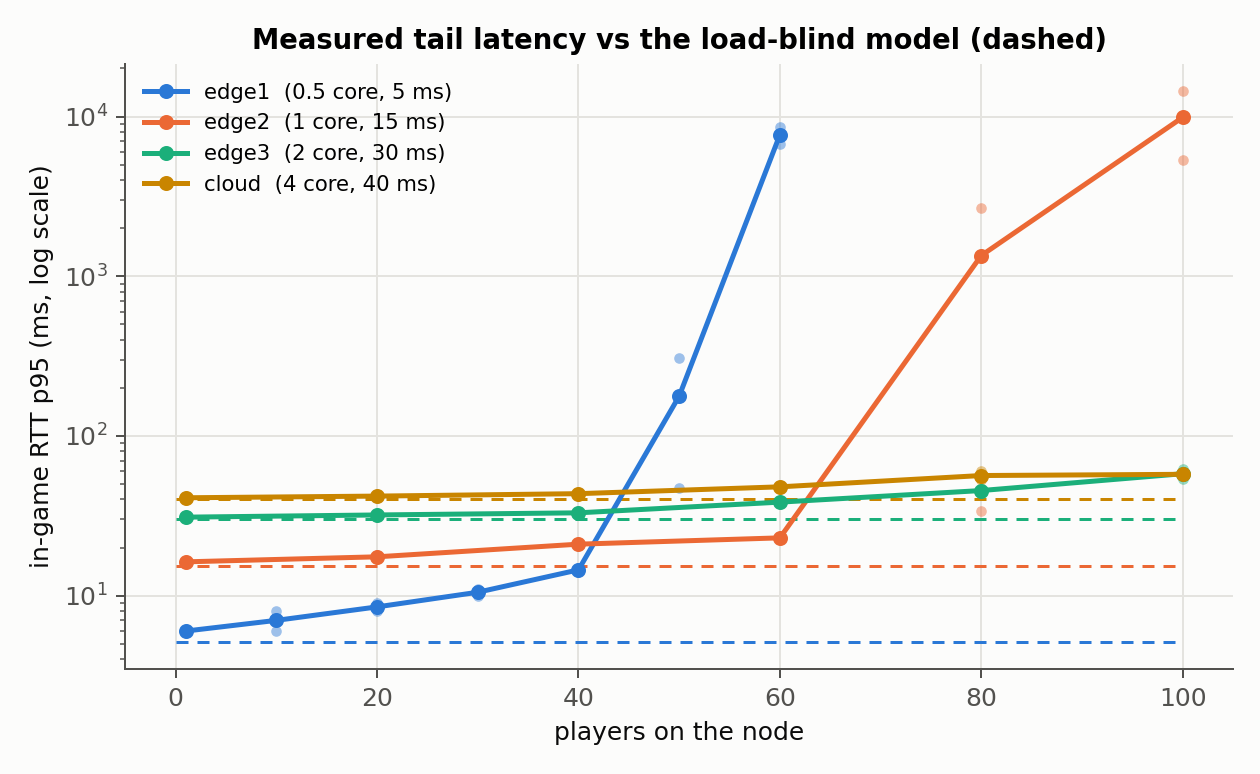
\includegraphics[width=\columnwidth]{fig1_p95_vs_players.png}
\caption{Measured p95 in-game RTT per node (solid; dots are the two
replicates) against the load-blind model's prediction (dashed).}
\label{fig:grid}
\end{figure}

\subsection{Rank inversion}
For a single match, the analytical model always picks edge1. That is correct
up to 40 players (edge1 14.5\,ms, edge2 21\,ms) and wrong at 60, where edge1
measures 7.7\,s and edge2 23\,ms: a regret of 7.66\,s on the worst player.
Both load-aware models switch to edge2 at 60 and have zero regret at every
measured load.

\subsection{Prediction error}
Table~\ref{tab:pred} fits each model on one replicate and predicts the other.
The learned model has the lowest median and mean error; the queueing model is
accurate in the flat region but its $1/(1-u)$ term explodes near the knee, giving a large mean
error. Fitted on three nodes and tested on the fourth, the learned model
transfers best to edge1, edge3 and cloud, and the queueing model to edge2.
On a third replicate measured hours later and never used in any fit (25
cells), the ranking holds: median error 1.2\,ms learned, 2.3\,ms queueing,
6.9\,ms analytical. Asked whether a cell breaks a 50\,ms budget, the learned
model scores F1 0.92 (all six violations caught), the queueing model 0.67 and
the analytical model 0, since it never predicts a violation.

\begin{table}[t]
\centering
\caption{Cross-replicate prediction error, 50 cells}
\label{tab:pred}
\begin{tabular}{lrrr}
\toprule
model & median abs. err. & factor off & MAE \\
\midrule
analytical & 5.8 ms & 2.82$\times$ & 768 ms \\
queueing   & 1.8 ms & 1.85$\times$ & 6547 ms \\
learned    & 0.9 ms & 1.28$\times$ & 469 ms \\
\bottomrule
\end{tabular}
\end{table}

\section{Placement Evaluation}

\textbf{Problem.} A batch of 40, 80, 120 or 160 players in matches of ten is
split across the four nodes to minimise the worst player's predicted p95. For
each model the optimum is found by exhaustive search.

\textbf{Deployment.} Every resulting placement is deployed on the testbed with
all loaded nodes running at once, and measured with the same streams as the
grid. No model's prediction is used to grade any model.

\begin{table}[t]
\centering
\caption{Worst node's measured p95 (ms) for each model's placement
(edge1/edge2/edge3/cloud players)}
\label{tab:deploy}
\setlength{\tabcolsep}{3.5pt}
\begin{tabular}{rlll}
\toprule
players & analytical & queueing & learned \\
\midrule
40  & 26 (40/0/0/0)        & 26 (40/0/0/0)  & 26 (40/0/0/0) \\
80  & 29\,897 (80/0/0/0)   & 20 (40/40/0/0) & 20 (40/40/0/0) \\
120 & 17\,758 (100/20/0/0) & 31 (40/80/0/0) & 32 (40/70/10/0) \\
160 & 19\,990 (100/60/0/0) & 35 (40/80/40/0) & 39 (40/70/50/0) \\
\bottomrule
\end{tabular}
\end{table}

\textbf{Result.} Table~\ref{tab:deploy} and Fig.~\ref{fig:deploy}. The
analytical model predicts 5--15\,ms for every scenario and fills the nearest
node to its 100-player cap before using the next; from 80 players its worst
players wait 18--30\,s, about 510 to 1500 times longer than under either
load-aware placement. Both load-aware
models keep edge1 at 40 players and spread the rest; their placements measure
within 4\,ms of each other, and the learned model's predictions of its own
deployments are within 1--12\,ms. On these scenarios the learned model's
advantage is in prediction, not in the placement decision: a correctly fitted
closed form reaches almost the same placement.

\begin{figure}[t]
\centering
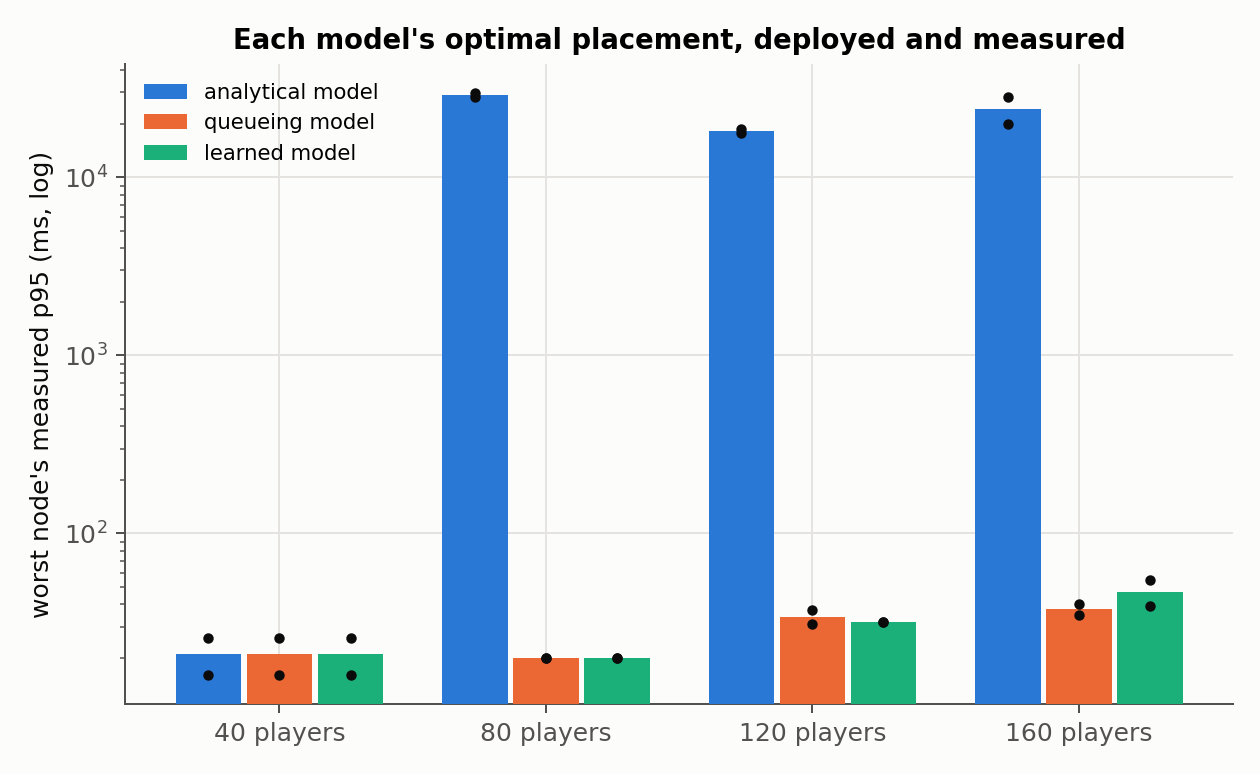
\includegraphics[width=\columnwidth]{fig5_deployments.png}
\caption{Each model's optimal placement, deployed and measured (log scale).}
\label{fig:deploy}
\end{figure}

\section{Closed-Loop Placement on the Testbed}

The deployments above are static: one placement, measured once. We also ran
placement as a controller on the live testbed. Every 2\,s it reads every
bot's latency samples, and every 5\,s every server's player count, tick time
and CPU; every 10\,s it may move one match (ten players) if the move lowers
the predicted worst-player p95 by at least 10\,ms and 20\%, or leaves it
unchanged and lowers the mean by 3\,ms, with a 60\,s cooldown per match. A move stops the match on one server and starts it on
another, so its players reconnect. New matches land on the nearest node with
room, as a distance-based matchmaker would place them, so two runs differ only
in the model that drives the controller.

\textbf{Same schedule, two controllers.} A match of ten players arrives
every 25\,s up to 140 players, holds for 150\,s, and leaves until 60 remain
(13\,min). Table~\ref{tab:live} and Fig.~\ref{fig:live}. The analytical
controller never moves a match: edge1 fills to 100 players and its p95 stays
above 10\,s until departures empty it. The learned controller keeps the
worst player's p95 at a median of 33\,ms; its remaining excursions over
100\,ms are the 10--25\,s after each new match lands on edge1 and before it
is moved away. Scored on the analytical run's own 10\,s windows, the models'
predictions of whether a node breaks 100\,ms reach F1 0.00 (analytical),
0.87 (queueing and learned) and 0.95 for a variant of the learned model that
corrects itself from live measurements.

\begin{table}[t]
\centering
\caption{Live controller, same 13-minute schedule (worst node's p95)}
\label{tab:live}
\setlength{\tabcolsep}{3.5pt}
\begin{tabular}{lrrrr}
\toprule
controller & median & max & over 100\,ms & moves \\
\midrule
analytical & 1\,058\,ms & 19.6\,s & 53\% & 0 \\
learned    & 33\,ms     & 817\,ms & 18\% & 10 \\
\bottomrule
\end{tabular}
\end{table}

\begin{figure}[t]
\centering
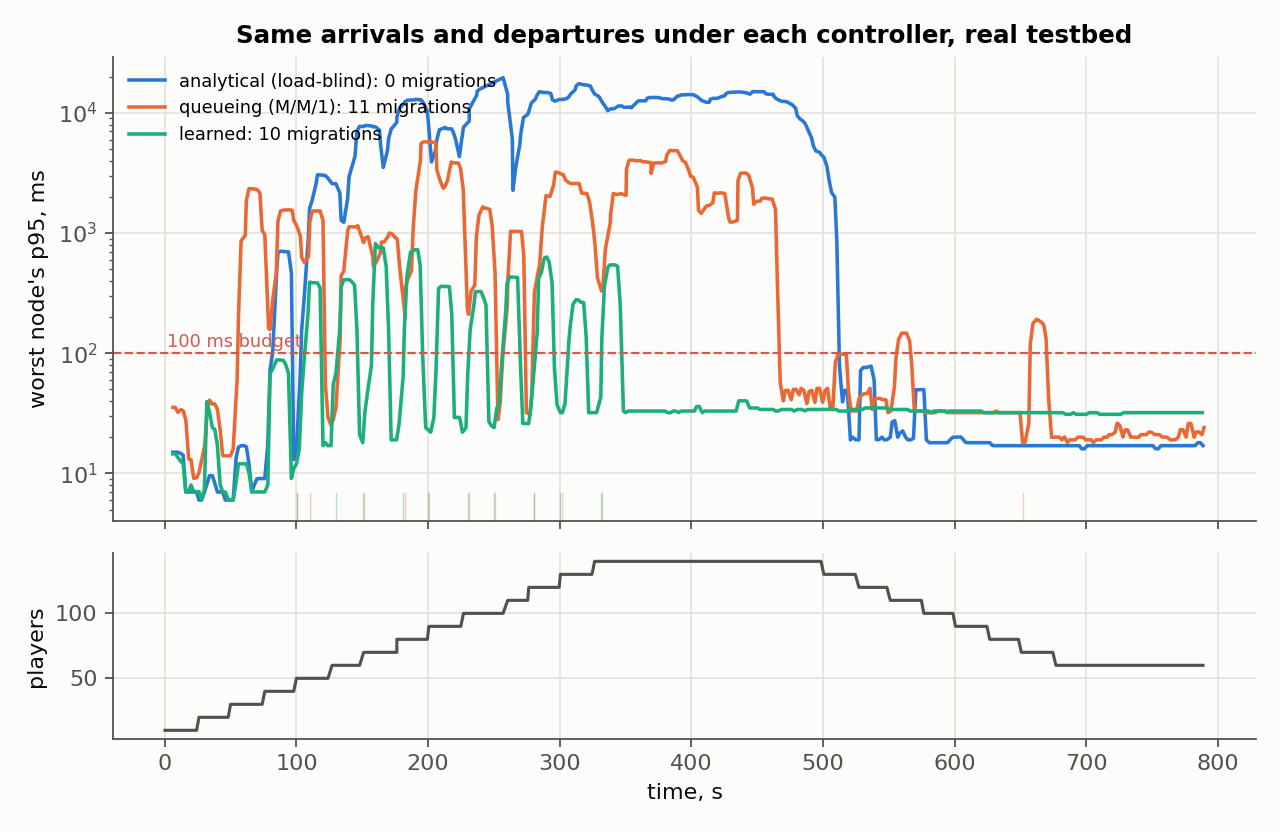
\includegraphics[width=\columnwidth]{fig6_live_ab.png}
\caption{Worst node's p95 over time under each controller, same arrivals and
departures (bottom). Ticks mark the learned controller's migrations.}
\label{fig:live}
\end{figure}

\textbf{A node gets slower and no model is told.} With eight matches
settled, edge1's CPU quota is cut from 0.5 to 0.25 cores at 220\,s
(Fig.~\ref{fig:drop}). The offline learned model still predicts edge1's
0.5-core curve: it keeps 40 players there and edge1's p95 stays at
0.2--2.6\,s for the remaining five minutes (99\% of the time over 100\,ms).
A variant corrects the model while it runs: each steady 10\,s window updates a
per-node factor $c$ such that the node at $P$ players behaves like the grid's
node at $cP$. Its first version noticed the cut and moved two matches off
within 70\,s, but light, healthy windows below the new knee pulled $c$ back
down and it moved a match back, which then saw 3.9\,s. With a five-minute
memory of loads measured over budget, a rerun was over 100\,ms for 4\% of
the time after the cut (the 15--20\,s before its first move) and never
reloaded edge1. The memory was added after the first run and each version ran
once; it shows the mechanism, not a tuned result.

\begin{figure}[t]
\centering
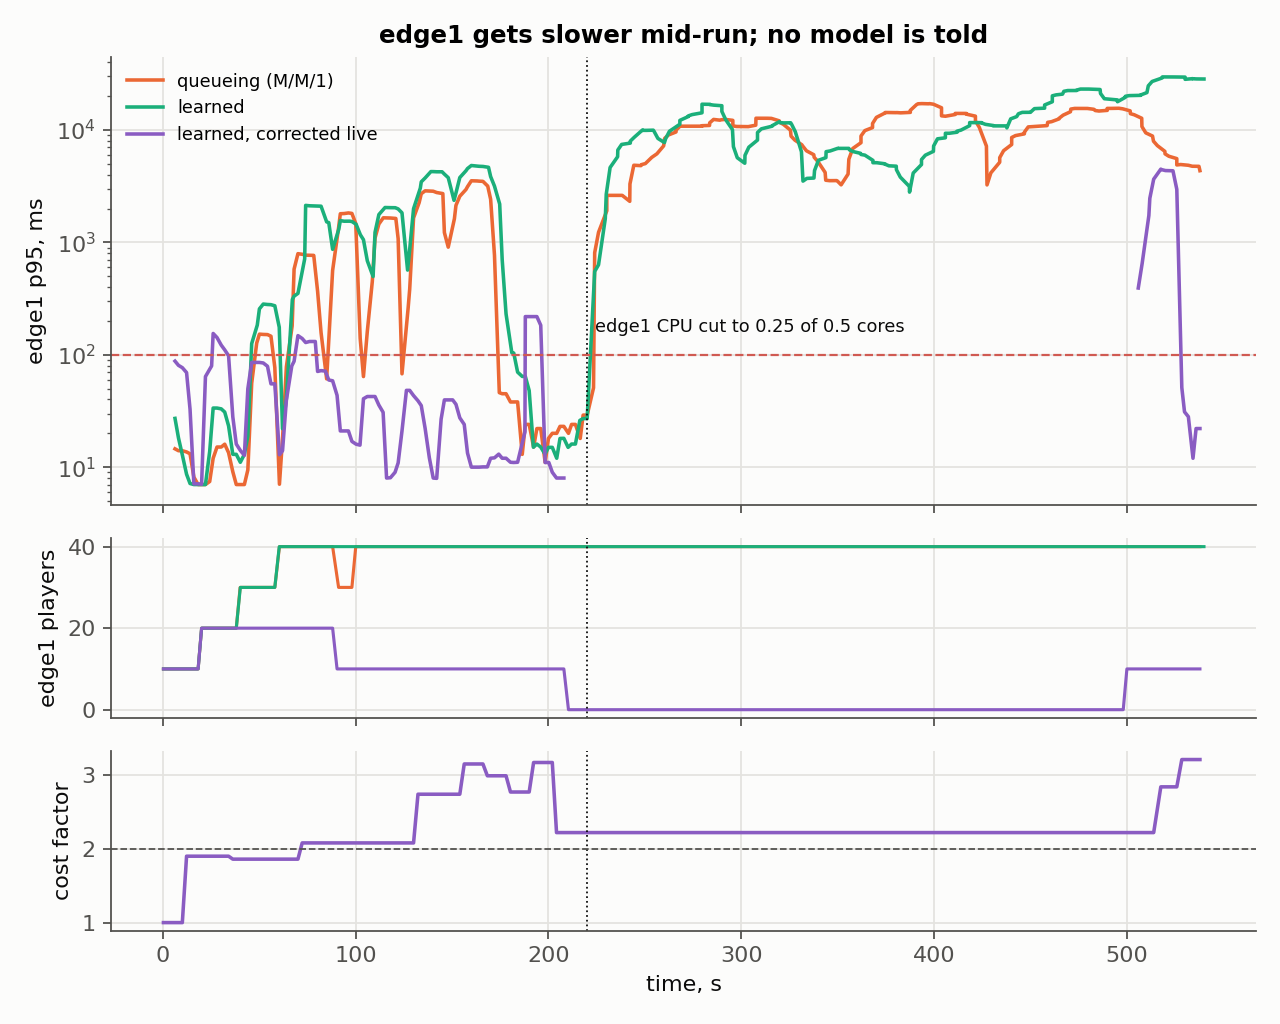
\includegraphics[width=\columnwidth]{fig7_live_capacity_drop.png}
\caption{edge1's CPU halved at 220\,s (dotted). Top: edge1's p95 under the
offline and the live-corrected learned model. Middle: players each leaves on
edge1. Bottom: the live model's cost factor for edge1 (true value after the
cut: 2).}
\label{fig:drop}
\end{figure}

\section{Threats to Validity}

\textbf{One host, three replicates.} All nodes share one laptop; three replicates
give a spread, not a confidence interval. At the knees the replicates differ
by 6--80$\times$, so the exact player count of a knee is not established.

\textbf{Host power mode.} A node capped at half a core runs in short
bursts, so the CPU governor keeps its clock low unless the host is in its
performance power mode. All clean runs used that mode. In the balanced mode
the same players cost 2--3$\times$ the CPU (edge1 with 20 players: 42\% of a
core instead of 14--18\%) and edge1's knee fell below 20 players. One edge1
pass and one full replicate were spoiled this way; they are excluded and kept
as evidence. The same node, players and network, changed only by a setting no
latency formula sees, moved the knee threefold.

\textbf{Chosen, not discovered, capacities.} The core counts and delays were
picked to create the trade-off. The claim is that an inversion exists, is
large, and is avoided by a load-aware model, not that edge nodes fail at a
particular player count. The 100-players-per-core capacity the queueing model
uses is untested above one core.

\textbf{Synthetic workload.} Bots walk and chat on a fixed schedule, and
hostile mobs are disabled; real players and real mob AI add load of other
shapes. The placement comparison covers four scenarios on four nodes; larger
problems are where the load-aware models could differ.

\section{Conclusion}

The load-blind latency model used to rank edge nodes is accurate only below a
node's saturation point, and above it the error is not a few milliseconds but
seconds: deployed, its placements left the worst players waiting 18--30\,s
where a load-aware placement measured 20--39\,ms on the same hardware. A model
learned from measurements predicts latency best, while on these scenarios a
fitted M/M/1 term already makes the right placement. Run live on the same
schedule, a load-blind controller never moves a match while a load-aware one
keeps the worst players at a median of 33\,ms, and a node that silently slows
down is handled only by a model that keeps learning from measurements and
remembers the loads it has seen fail. The practical
lesson is
that the latency term in placement must see load, and that its shape is
better measured than assumed. Future work: more replicates on dedicated
hardware, nodes pushed past their knees at higher core counts, larger
placement problems, state handover instead of reconnection, and network
impairments that make the bandwidth term
non-trivial. Code, raw measurements and the dataset:
\url{https://github.com/ankamteja/latency-aware-edge-game-placement}.

\bibliographystyle{IEEEtran}
\bibliography{refs}

\end{document}
